\documentclass[tikz,border=9pt]{standalone}
\usepackage{amsmath,amssymb}
\usetikzlibrary{arrows.meta,positioning,calc}
\begin{document}
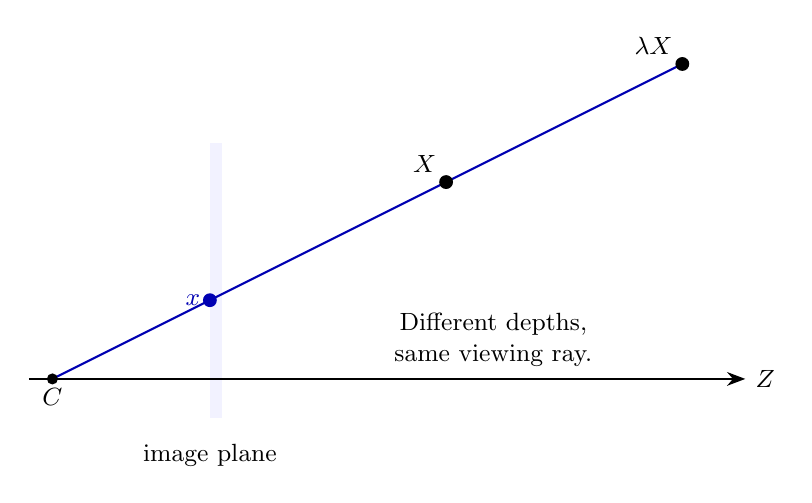
\begin{tikzpicture}[font=\small,arr/.style={-{Stealth},thick},box/.style={draw=blue!55!black,rounded corners,fill=blue!4,align=center,text width=2.9cm,minimum height=1.05cm}]

\coordinate (C) at (0,0);\coordinate (X) at (5,2.5);\coordinate (Y) at (8,4);
\fill[blue!5] (2,-.5) rectangle (2.15,3);
\draw[arr] (-.3,0)--(8.8,0) node[right]{$Z$};
\draw[thick,blue!70!black] (C)--(Y);
\fill (C) circle(2pt) node[below]{$C$};
\fill[blue!70!black] (2,1) circle(2.5pt) node[left]{$x$};
\fill (X) circle(2.5pt) node[above left]{$X$};
\fill (Y) circle(2.5pt) node[above left]{$\lambda X$};
\node[below,align=center] at (2,-.7){image plane};
\node[align=center] at (5.6,.5){Different depths,\\same viewing ray.};

\end{tikzpicture}
\end{document}
